\section{Introduction}
\label{sec:intro}

Knowledge distillation (KD) has become a standard technique for compressing deep neural networks, enabling deployment of efficient models on resource-constrained platforms \cite{hinton2015distilling}. In object detection, KD allows lightweight student networks to acquire knowledge from larger, more accurate teacher models, achieving comparable performance with reduced computational cost \cite{chen2017learning, dai2021general}. However, the reliability of KD under adverse visual conditions---particularly visibility degradation caused by fog, haze, or rain---remains a critical open question.

Recent studies have documented that KD performance degrades under domain shift and adverse weather conditions \cite{guo2021meets, du2022learning}. Yet the \\\emph{why} remains unclear. Does KD fail because teacher-student distribution alignment breaks down? Does teacher uncertainty amplify under degraded inputs? Or does visibility disruption fundamentally alter the visual cues that knowledge transfer depends upon? Without understanding the dominant failure mechanism, efforts to develop robust KD methods risk addressing symptoms rather than causes.

This paper addresses this gap through a mechanism-driven empirical study. Rather than proposing yet another KD variant, we systematically dissect why existing KD approaches fail under visibility degradation. Our methodology employs a structured branch-wise analysis: we isolate four distinct KD mechanisms---logit distillation, feature distillation, attention distillation, and localization distillation---and evaluate their behavior across a controlled spectrum of visibility levels.

Our study yields three principal findings. First, we confirm that branch-wise performance structure exists: different KD branches respond distinctly to visibility degradation, with logit distillation proving suboptimal despite its prevalence in the literature, and localization distillation demonstrating relative robustness. Second, we empirically test three hypothesized failure mechanisms. Distribution mismatch and uncertainty amplification, while frequently invoked as explanations, show weak and statistically insignificant correlations with KD gains ($|r| < 0.5$, $p > 0.7$), indicating insufficient explanatory power in our setting. Third, and most critically, we identify occlusion---a specific, measurable component of visibility degradation---as exhibiting strong negative correlation with localization performance ($r=-0.989$, $p=0.0015$), representing the most directly supported mechanism among those tested.

These findings carry significant methodological implications. Our analysis indicates that logit KD failure is unlikely to be resolved through simple hyperparameter adjustment alone. The strong relationship between occlusion and localization performance suggests that future KD methods for adverse conditions should prioritize mechanisms that explicitly handle occlusion and spatial information loss, rather than focusing solely on distribution alignment or uncertainty calibration.

The contributions of this paper are:
\begin{itemize}
    \item We provide the first controlled empirical study that disentangles competing explanations for KD failure under visibility degradation, establishing a structured observation-mechanism validation framework;
    \item We show that widely assumed mechanisms---distribution mismatch and uncertainty amplification---do not sufficiently explain observed KD degradation, challenging prevailing intuitions in the literature;
    \item We identify occlusion, as a specific and measurable component of visibility degradation, as the most directly supported factor among those tested;
    \item We demonstrate that KD failure is not attributable to simple hyperparameter tuning, indicating fundamental limitations that require architectural rather than configurational solutions.
\end{itemize}

Beyond the specific KD research community, this study addresses a practical concern in intelligent transportation and all-weather visual perception systems. Model compression through KD is frequently required for deploying detection networks on edge devices with limited computational resources; understanding why KD fails under visibility degradation is essential for building robust perception pipelines that operate reliably across varying environmental conditions. From this perspective, the paper contributes not only to detection methodology but also to the broader domain of image communication and visual perception robustness.

\Cref{fig:conceptual_framework} illustrates our mechanism-driven analysis approach.

\begin{figure*}[htbp]
\centering
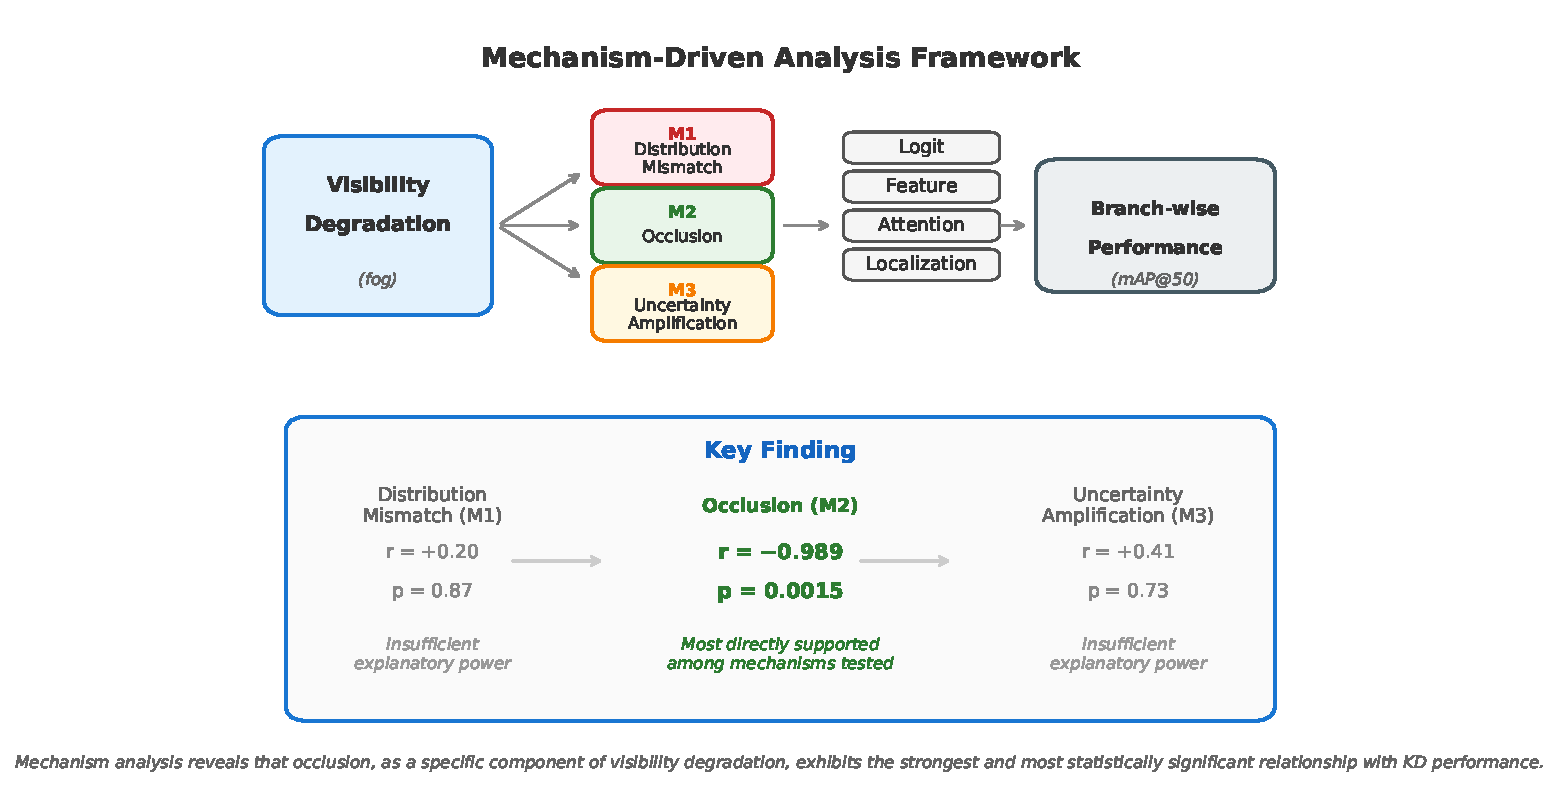
\includegraphics[width=0.9\textwidth]{figures/fig1_mechanism_framework.pdf}
\caption{Mechanism-driven analysis framework. We evaluate three hypothesized mechanisms (M1, M2, M3) across four KD branches to identify the most strongly supported factor among those tested. Our findings indicate that occlusion (within M2) is the most directly supported mechanism, while distribution mismatch and uncertainty amplification show insufficient explanatory power.}
\label{fig:conceptual_framework}
\end{figure*}

The remainder of this paper is organized as follows. \cref{sec:related} reviews related work on KD for detection and under domain shift. \cref{sec:setup} describes our experimental design and branch-wise framework. \cref{sec:observation} presents the structured observation results establishing branch-wise performance structure. \cref{sec:mechanism} details our mechanism analysis and the evidence identifying occlusion as the most directly supported mechanism. \cref{sec:discussion} discusses implications and limitations, and \cref{sec:conclusion} concludes with future directions.
